\documentclass[10pt]{beamer}

%%%
% PREAMBLE FOR THIS DOC 
%%%
%https://tex.stackexchange.com/questions/68821/is-it-possible-to-create-a-latex-preamble-header
\usepackage{/Users/miw267/Repos/csci246_fall2025/slides/preambles/beamer_preamble_for_CSCI246}



%%% TRY TO RESHOW TOC AT EACH SECTION START (with current section highlighted)
% Reference: https://tex.stackexchange.com/questions/280436/how-to-highlight-a-specific-section-in-beamer-toc
\newcommand\tocforsect[2]{%
  \begingroup
  \edef\safesection{\thesection}
  \setcounter{section}{#1}
  \tableofcontents[#2,currentsection]
  \setcounter{section}{\safesection}
  \endgroup
}


%%%% HERES HOW TO DO IT CORRECTLY
% FIRST IN .STY FILE, DO
%\usetheme[sectionpage=none]{metropolis}
% THEN AT EACH SECTION DO
%\begin{frame}{Outline}
%  \tableofcontents[currentsection]	
%\end{frame}



%\setbeamertemplate{navigation symbols}{}
%\setbeamertemplate{footline}[frame number]{}


%%%
% DOCUMENT
%%%

\begin{document}

%\maketitle

%% Title page frame
%\begin{frame}
%    \titlepage 
%\end{frame}





\title{09/14/2026: Factorial}
\author{CSCI 246: Discrete Structures}
\date{Textbook reference: Sec. 9, Scheinerman}

\begin{frame}
    \titlepage 
\end{frame}


\begin{frame}
\small 
\begin{mygreenbox}[title=Graded Quiz Pickup]
Quizzes are in the front of the room, grouped into four bins (A-G, H-L, M-R, S-Z) by last name. The quizzes are upside down with your last name on the back. Come find yours before, during, or after class.  Only turn the quiz over if it's yours.
\end{mygreenbox} 

\vfill 


\begin{myyellowbox}[title=Today's Agenda]
\begin{itemize}
	\item Quiz feedback/logistics ($\approx$ 10  mins)
	\item Review group exercises ($\approx$ 10 mins)
	\item Mini-lecture  ($\approx$  15 mins)
	\item Group exercises $\approx$  15 mins)
\end{itemize}

\end{myyellowbox}
\vfill 

\end{frame}


\begin{frame}[standout]
Quiz feedback/logistics
\end{frame}




\begin{frame}{Weekly Quiz \#2: Scores}

\begin{figure}[ht]
        \centering
        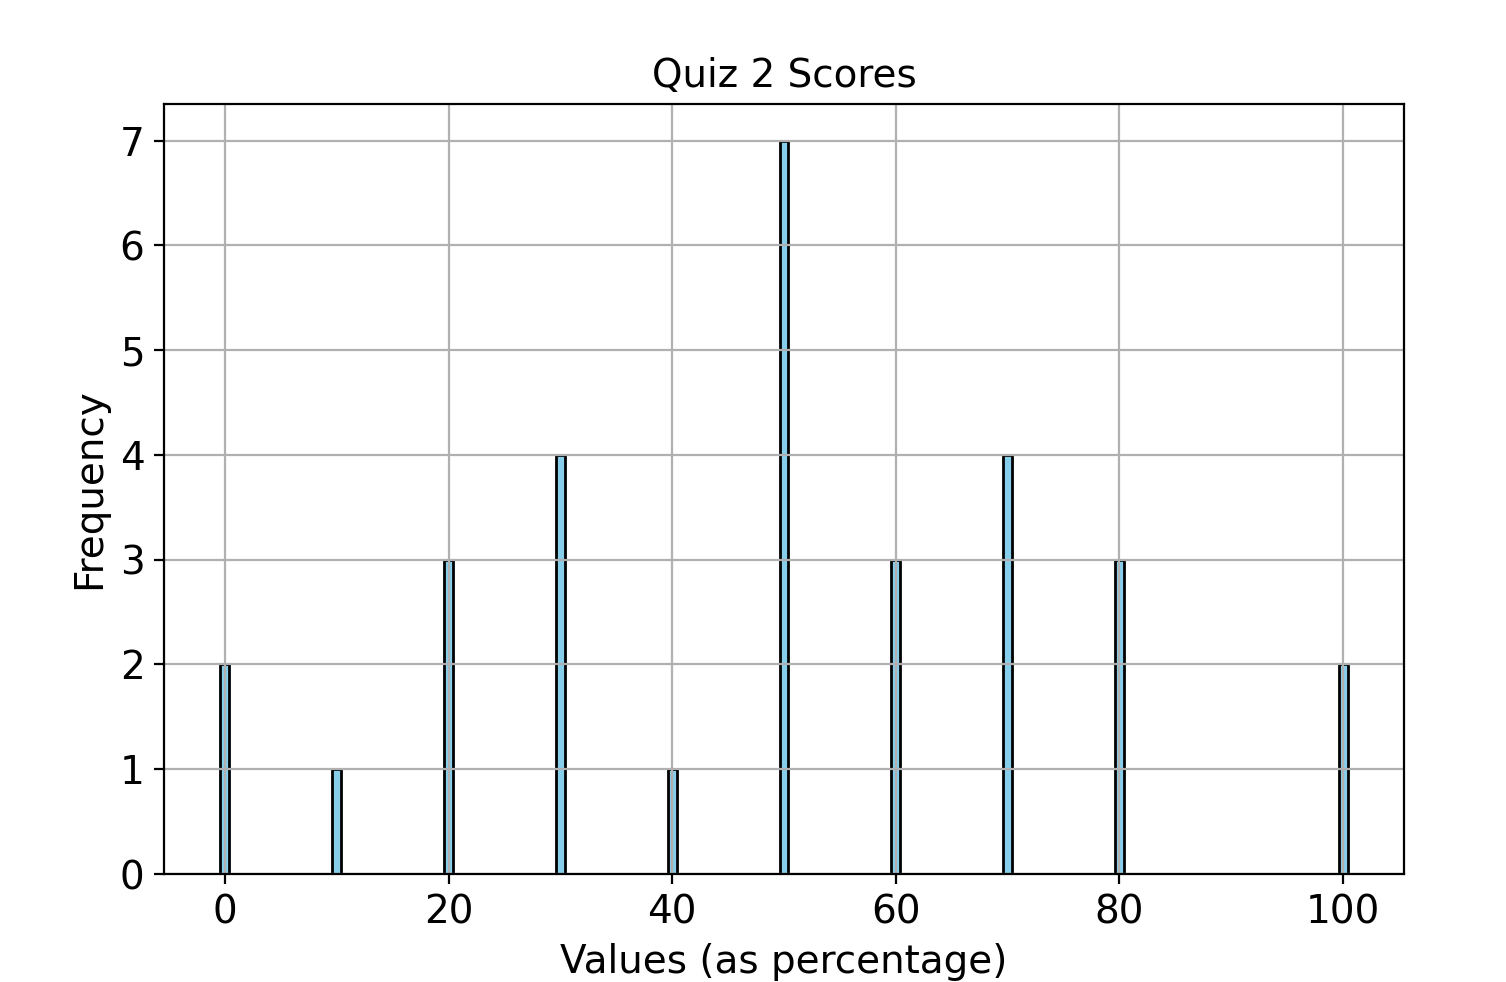
\includegraphics[width=\textwidth]{images/quiz_2_scores}
        \small Median: 2.5/5 (50\%).
\end{figure}
\vfill 

\end{frame}




\begin{frame}
\begin{myyellowbox}[title=Proofs: A second pass]
I've added an extra day before the midterm to review proofs, with an option to retake quiz \#2.
\end{myyellowbox}

\vfill 
\pause 

\begin{mygreenbox}[title=Resources for help]
\begin{enumerate}
\item Madhav and I each have three office hours weekly.  Try writing up a proof and bringing it to show us. \pause 
\item (New!) \textbf{Free} daily tutoring is provided by SmartyCats. You can make an appointment Mon-Fri 3:30-5:30.  See the updated \href{https://github.com/mikewojnowicz/csci246_fall2026/blob/main/syllabus/syllabus.pdf}{\underline{\blue{syllabus}}}. \pause 
\item (New!) Madhav (TA) is available to meet Friday mornings by appointment.
\end{enumerate}
\end{mygreenbox}	
\vfill 
\end{frame}



\begin{frame}{Weekly Quiz \#2: Scores - Updated}

I discarded the first question since I didn't provide the definition for odd. 
\begin{figure}[ht]
        \centering
        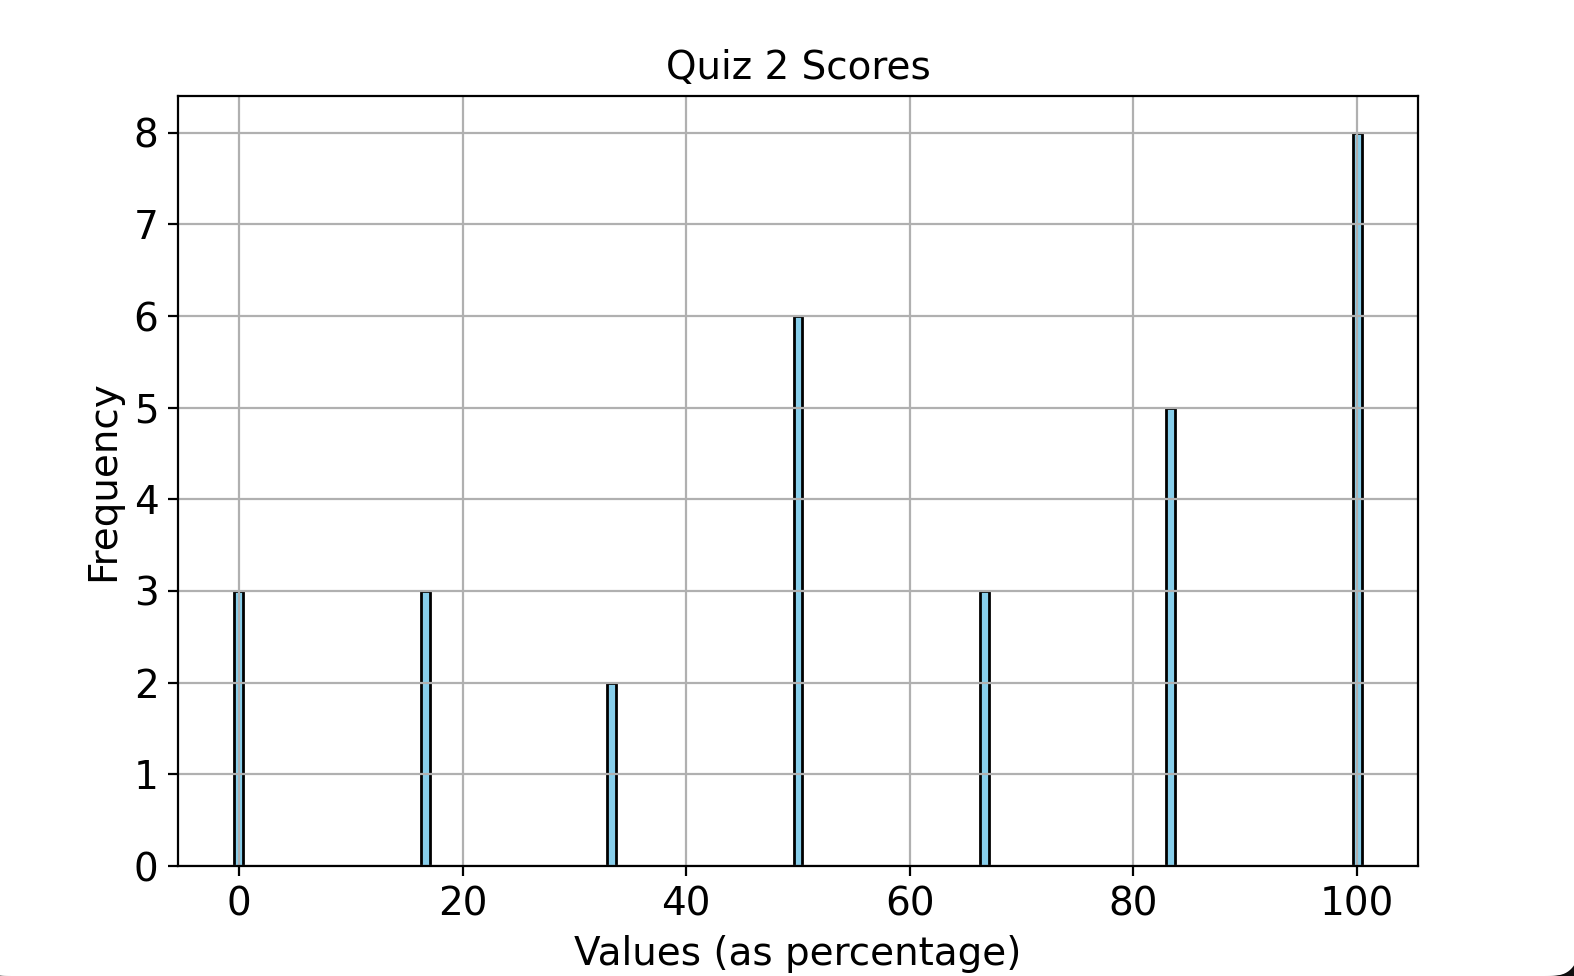
\includegraphics[width=\textwidth]{images/quiz_2_scores_updated}
        \small Median: 2/3(66)\%.
\end{figure}
\vfill 

\end{frame}

\begin{frame}

\begin{myredbox}[title=Quiz Logistics]

\begin{itemize}
\item Going forward, if you finish the quiz early, you will need to be \underline{silent} until everyone else is finished.  Violators will receive a zero. \pause 
\item Both quiz grades have been posted to Canvas. \pause 
\item The weekly quizzes are equally weighted.  The denominator is chosen for convenience.  \pause 
\item Quiz feedback has been posted to the repo.
\end{itemize}

\end{myredbox}	
\end{frame}





\begin{frame}[standout]
Review of lists
\end{frame}




\begin{frame}{Multiplication Principle}

\begin{center}
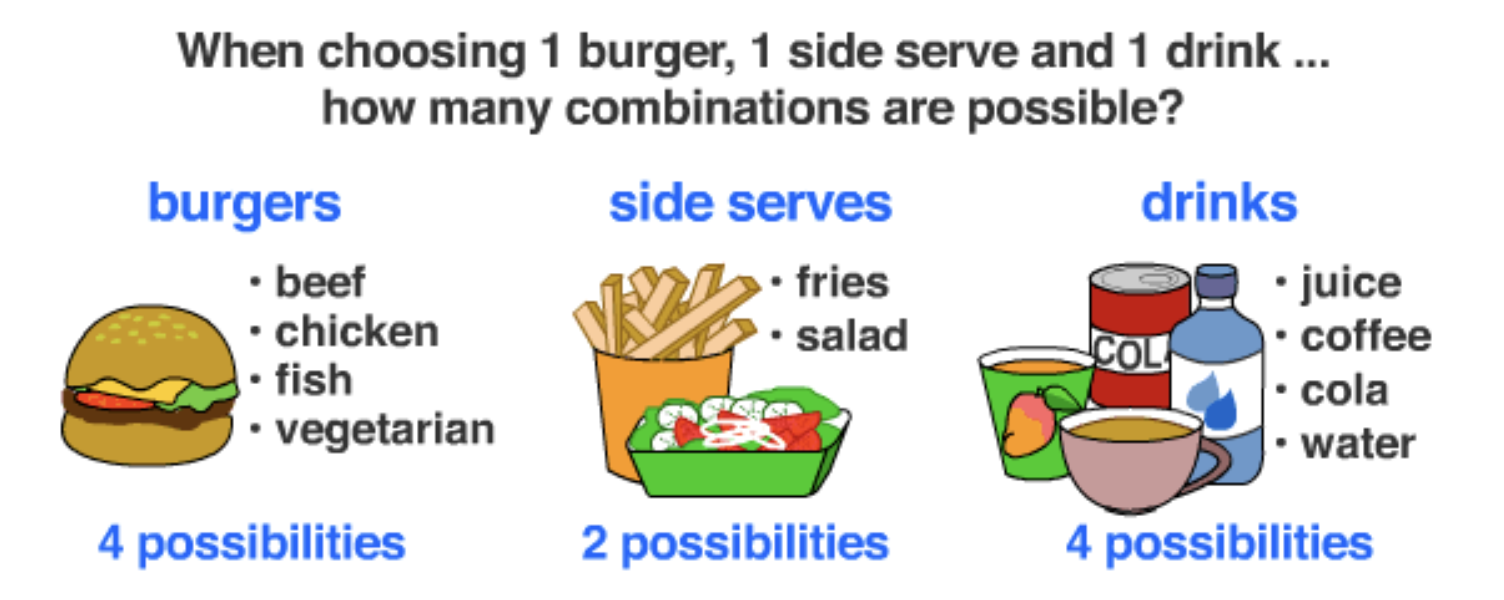
\includegraphics[width=\textwidth]{images/multiplication_principle.png}
\Large \colorbox{blue!30}{\textbf{Solution.}} \blue{There are $4 \times 2 \times 4 = 32$ possibilities.}
\end{center}
\end{frame}

\begin{frame}{Multiplication principle}
\begin{mygreenbox}[title= \textbf{Multiplication Principle} (Theorem 8.2 from Scheinerman)]
Consider the two-element lists for which there are $n$ choices for the first element, and for each choice of the first element there are $m$ choices for the second element. Then the number of such lists is $nm$.
\end{mygreenbox}
\vfill 
\colorbox{red!30}{\textbf{Remark.}} We can apply the multiplication principle \alert{iteratively}.   So, for example, if we want to form three-element lists for which there are $n$,$m$, and $k$ choices for the 1st, 2nd, and 3rd elements respectively, then there are $nmk$ such lists. 
\end{frame}


\begin{frame}{Multiplication principle with constant pool size}

\begin{mygreenbox}[title= Theorem 8.6 from Scheinerman]
The number of lists of length $k$ whose elements are chosen from a pool of $n$ elements 
%
\begin{align*}
= \begin{cases}
 n^k, & \text{if repetitions are permitted} \\
 (n)_k, & \text{if repetitions are forbidden}	
 \end{cases}
\end{align*}
\end{mygreenbox}

\vfill 

\colorbox{red!30}{\textbf{Notation.}}
\[  (n)_k \defeq \explaintermbrace{$k$ terms}{n \times (n-1) \times \cdots \times (n-k+1)}\]

\end{frame}




\begin{frame}{Multiplication principle with constant pool size}

\colorbox{yellow!30}{\textbf{Example: Lottery}} Suppose we draw $k=6$ balls from the jar of $n=10$ balls and record the sequence in which they appear. How many possible sequences are there?

\begin{center}
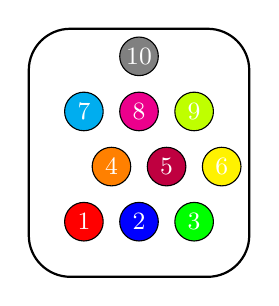
\begin{tikzpicture}[scale=0.7, every node/.style={font=\small, white}]
% Jar outline
\draw[thick, rounded corners=15pt] (0,0) rectangle (4,4.5);

% Balls (10 different colors + numbers)
\foreach \x/\y/\c/\n in {
  1/1/red/1,
  2/1/blue/2,
  3/1/green/3,
  1.5/2/orange/4,
  2.5/2/purple/5,
  3.5/2/yellow/6,
  1/3/cyan/7,
  2/3/magenta/8,
  3/3/lime/9,
  2/4/gray/10
} {
  % fill and draw circle
  \fill[\c] (\x,\y) circle (0.35);
  \draw (\x,\y) circle (0.35);
  % number on the ball
  \node at (\x,\y) {\n};
}
\end{tikzpicture}
\end{center}

\vfill 

\colorbox{green!30}{\textbf{Solution to Lottery Problem.}} The number of possible sequences if we draw $k=6$ balls from the jar of $n=10$ balls and record the sequence in which they appear is:
%
\begin{align*}
= \begin{cases}
 10^6, & \text{if repetitions are permitted} \\
 (10)_6 = 10 \cdot 9 \cdot 8 \cdot 7 \cdot 6 \cdot 5, & \text{if repetitions are forbidden}	
 \end{cases}
\end{align*}

\end{frame}





\begin{frame}[standout]
Factorial
\end{frame}



\begin{frame}
\colorbox{yellow!30}{\textbf{Poll.}} In how many different orders could these runners in the 2022 NYC marathon runners end up finishing the race?
\begin{center}
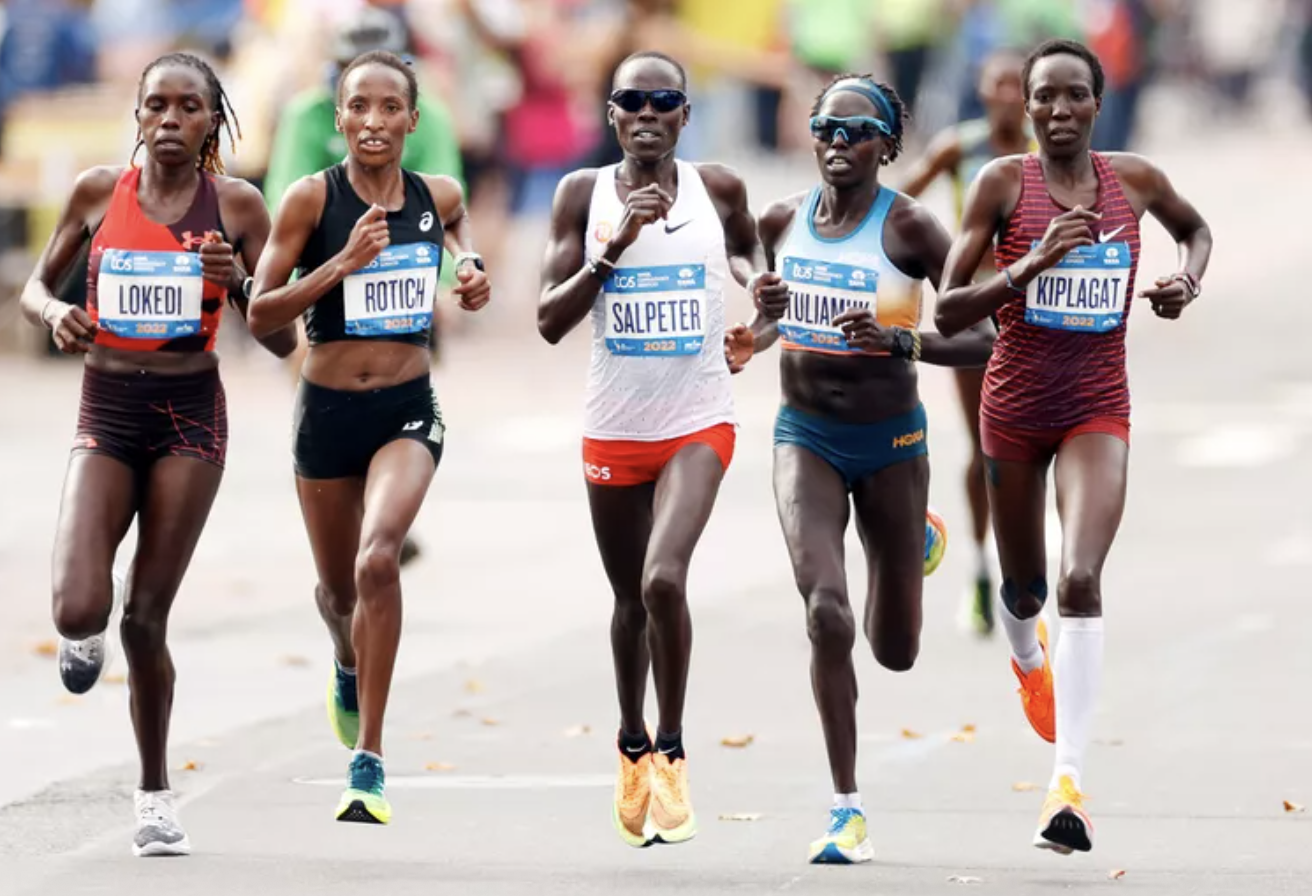
\includegraphics[width=.75\textwidth]{images/runners}	
\end{center}
\vfill \pause 

\colorbox{green!30}{\textbf{Solution.}} \only<2-3>{$5!$} \only<3>{What does that mean?} \only<4->{$5! = 5 \times 4 \times 3 \times 2 \times 1$.} 
\vfill \pause 
\colorbox{red!30}{\textbf{Explanation.}} \pause Why is this correct?  \pause Remember the \alert{multiplication principle}.  There are 5 choices for 1st place.  For each such choice, there are 4 choices for 2nd place.  Etc.  \pause This is like nested for loops!

\end{frame}



\begin{frame}{Factorial}

\begin{mygreenbox}[title=Definition]
\textbf{$n$ factorial}, written $n!$, is the number of length-$n$ lists that can be formed from a pool of $n$ objects in which repetition is forbidden. 
\end{mygreenbox}

\vfill 
\pause 

\begin{myredbox}[title=Technical Note]
 The definition implies that $n!$ is only defined when $n$ is a non-negative integer ($0,1,2,3,\hdots$).
\end{myredbox}

\vfill 
\pause 

\begin{myyellowbox}[title=Interpretation]
We can think of $n$-factorial as the number of way to \textbf{shuffle}  $n$ objects. \\

For example, $5! = 5 \times 4 \times 3 \times 2 \times 1 = 120$ is the number of ways we can order the NYC Marathon runners  \texttt{Sharon Lokedi, Caroline Rotich, Lonah Salpeter, Edna Kiplagat}, and     \texttt{Aliphine Tuliamuk}.
\end{myyellowbox}


\end{frame}


\begin{frame}{Falling Factorial}
\small 
\colorbox{red!30}{\textbf{Recall.}} Last time we defined the \textbf{falling factorial}

\[ (n)_k \defeq \explaintermbrace{$k$ terms}{n \times (n-1) \times (n-2) \times \cdots \times (n-k+1)}, \]

read as \textit{$n$ falling $k$}, as\only<1>{\alert{ (How to describe this this out loud?)}}\only<2->{ the product of $k$ consecutive integers starting from $n$ and decreasing by one each time.} \pause 

\vfill 
\pause 
\colorbox{yellow!30}{\textbf{Poll.}} How is the falling factorial related to the factorial?

\vfill 
\pause 
\colorbox{green!30}{\textbf{Solution.}} Note that
%
\begin{align*}
(n)_1 &= n \\
(n)_2 &= n \times (n-1) \\
(n)_3 &= n \times  (n-1) \times (n-2) \\
\vdots &= \vdots \\
(n)_n &= n \times (n-1) \times (n-2) \cdots \times 1
\end{align*}
%
Hence $n!=(n)_n$, and so the factorial is a special case of the falling factorial.

\end{frame}


\begin{frame}{Factorial: Special case of falling factorial}

\begin{mygreenbox}[title= Theorem 8.6 from Scheinerman]
The number of lists of length \only<1-2>{$k$}\only<3->{\red{\text{$k$}}} whose elements are chosen from a pool of $n$ elements 
%
\begin{align*}
= \begin{cases}
 n^k, & \text{if repetitions are permitted} \\
 \only<1-2>{(n)_k} \only<3->{\red{(n)_k}} & \text{if repetitions are forbidden}
 \end{cases}
\end{align*}
\end{mygreenbox}

\vfill 

\begin{mygreenbox}[title=Definition (from Scheinerman Sec. 9)]
The number of lists of length \only<1-2>{$n$}\only<3->{\red{\textbf{$n$}}} whose elements are chosen from a pool of  $n$ elements if repetitions are forbidden is called \textbf{$n$ factorial}, written\only<1-2>{ $n!$}\only<3->{\red{ $n!$}}.   
\end{mygreenbox}
\vfill 
\pause 
\colorbox{red!30}{\textbf{Note.}} The factorial is a special case of the falling factorial where \only<2>{\alert{what?}}\only<3->{the length of the list, $k$, equals the length of the pool of elements we're selecting from, $n$.} 
\end{frame}


\begin{frame}{Permutations and combinations}


Suppose you are counting the number of ways to do something...

\vfill 

% ------------------------------
% First row: Permutations
% ------------------------------
\begin{columns}[t] % top-align columns
    \column{0.7\textwidth}
    \textbf{Permutations} are what you use when the \underline{order matters}. 
    For instance, we may want to calculate the number of possible orderings 
    for the 5 marathon runners. For this, we can use factorials 
    (or more generally, falling factorials). \only<1>{\alert{(How so?)}}
    \column{0.3\textwidth}
    \vspace{0pt} % forces top alignment
    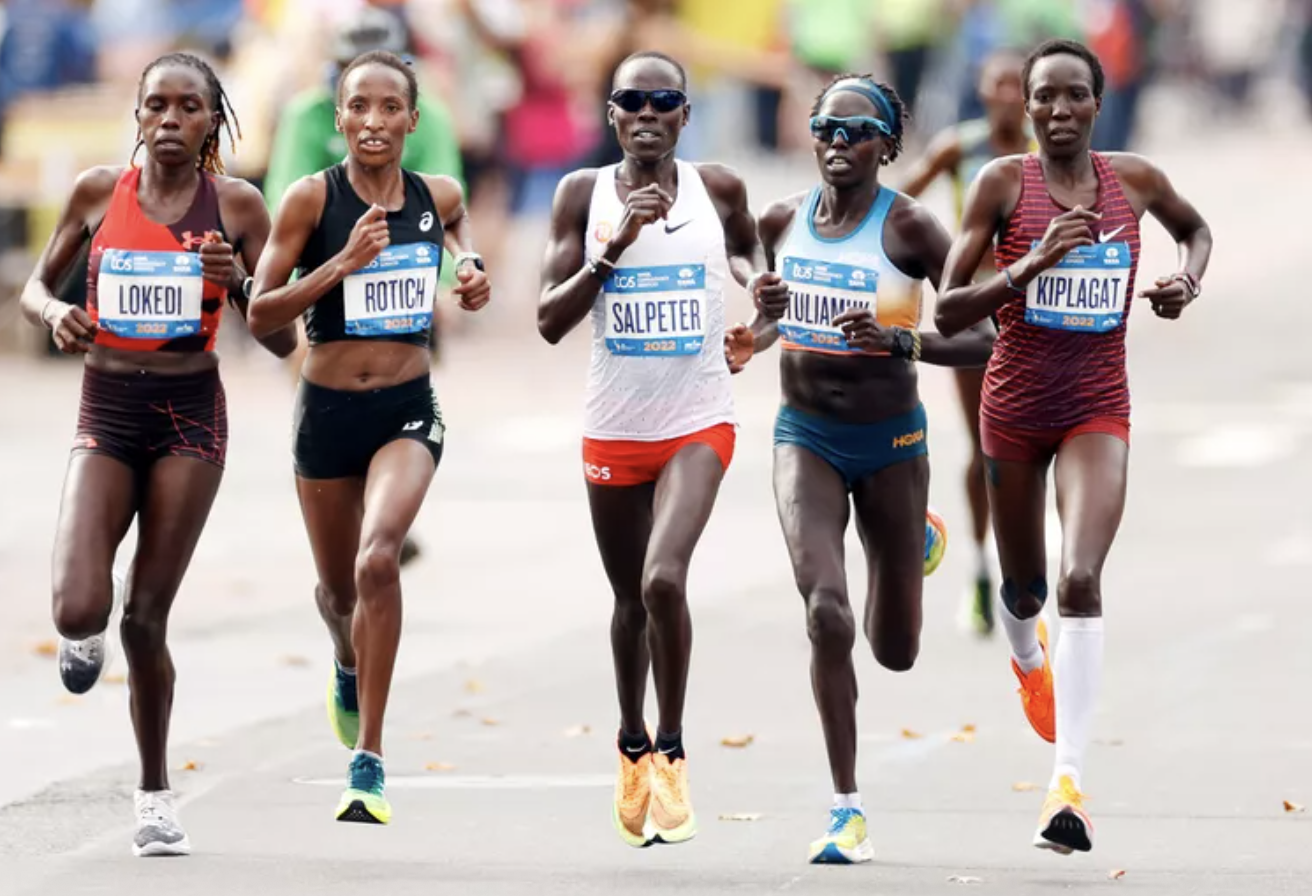
\includegraphics[width=\linewidth]{images/runners.png}
\end{columns}

\pause 
\vspace{1em} % space between rows

% ------------------------------
% Second row: Combinations
% ------------------------------
\begin{columns}[t] % top-align columns
    \column{0.7\textwidth}
    \textbf{Combinations} are what you use when the \underline{order doesn’t matter}. 
    For instance, if you have 10 different pieces of clothing you want to 
    take on a trip, but you can only fit 7 of them in your suitcase, it matters 
    which 7 you pick, but it doesn’t matter what order you put them in the suitcase.
    \column{0.3\textwidth}
    \vspace{0pt} % forces top alignment
    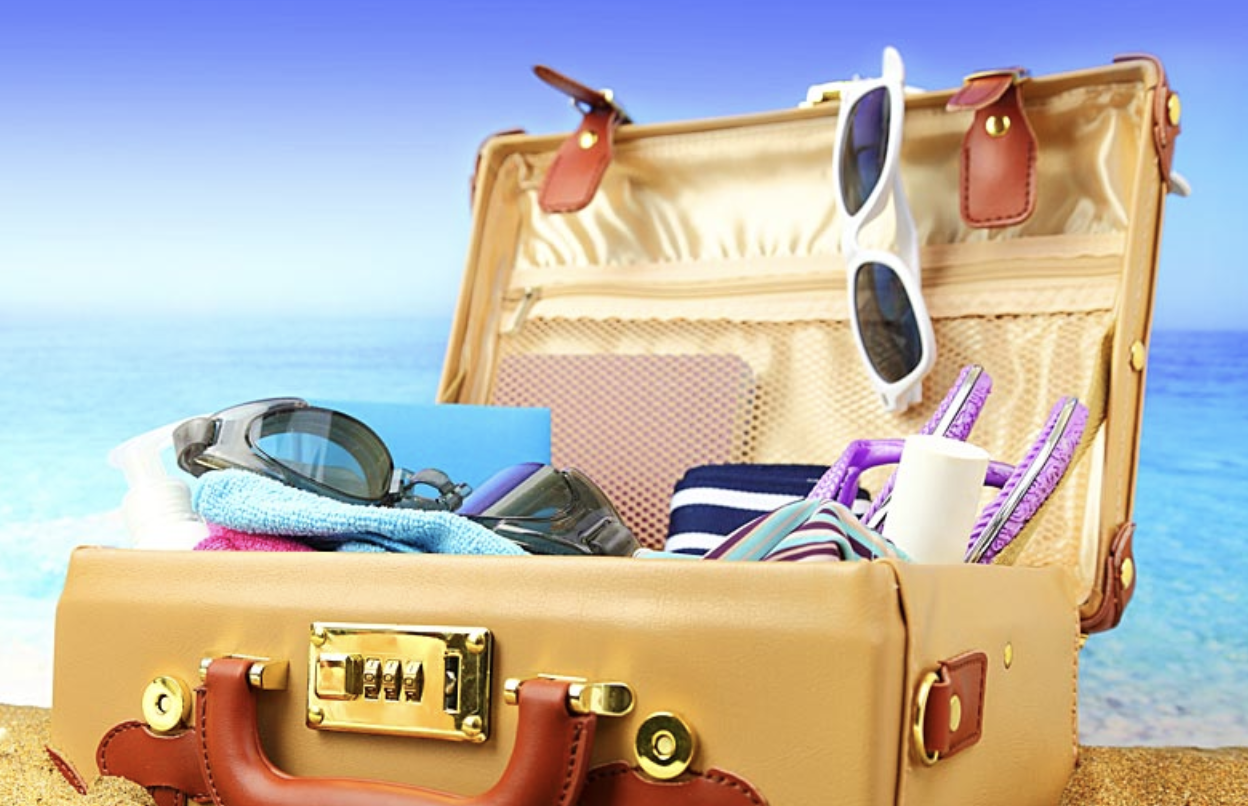
\includegraphics[width=\linewidth]{images/suitcase.png}
\end{columns}

\vfill 
\pause 

\colorbox{red!30}{\textbf{Relation to textbook.}} Right now we're working with permutations. (Note: we're working with lists, and lists are \alert{ordered!})  We'll get to combinations later, in Sec. 17 (Binomial Coefficients).
	
\end{frame}


\begin{frame}{Applications in computer science: Some examples}

\begin{columns}[t] % top-align columns
    \column{0.7\textwidth}
    \textbf{Graph algorithms.} Permutations are used when checking all possible paths. Example: the \alert{Traveling Salesman Problem}, where  a salesman must visit each city from a set (e.g. each U.S. capitol) exactly once and return to the starting city, finding the cheapest possible route to minimize travel cost. One  approach checks all 
$n!$ possible orderings of cities to find the cheapest tour.
    \column{0.3\textwidth}
    \vspace{0pt} % forces top alignment
    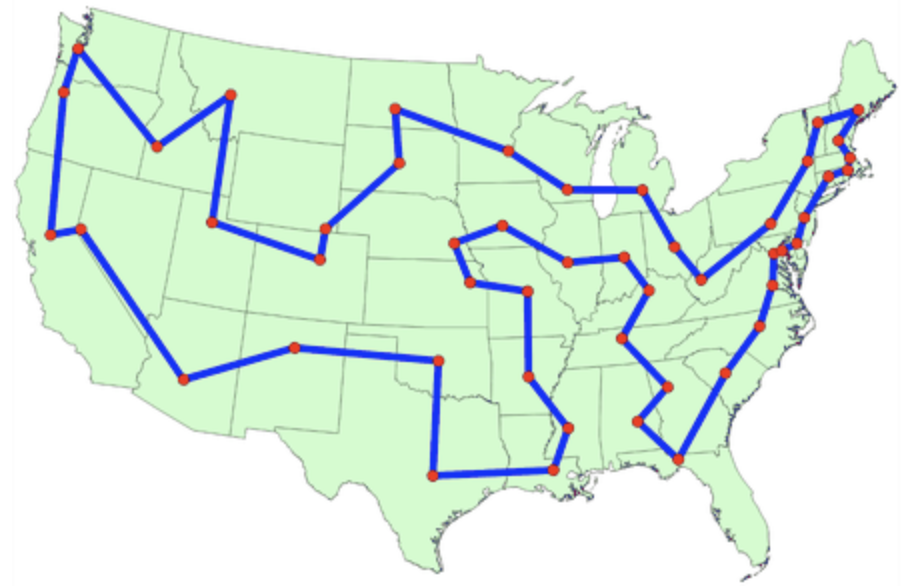
\includegraphics[width=\linewidth]{images/traveling_salesman}
\end{columns}

\pause 
\vspace{1em} % space between rows
\begin{columns}[t] % top-align columns
    \column{0.7\textwidth}
    \textbf{ Assigning IP addresses in a subnet.}   Suppose a network has $n$ available IP addresses and you want to assign $k$ devices distinct addresses. The number of ways to assign the addresses is $(n)_k$.
  \column{0.3\textwidth}
    \vspace{0pt} % forces top alignment
    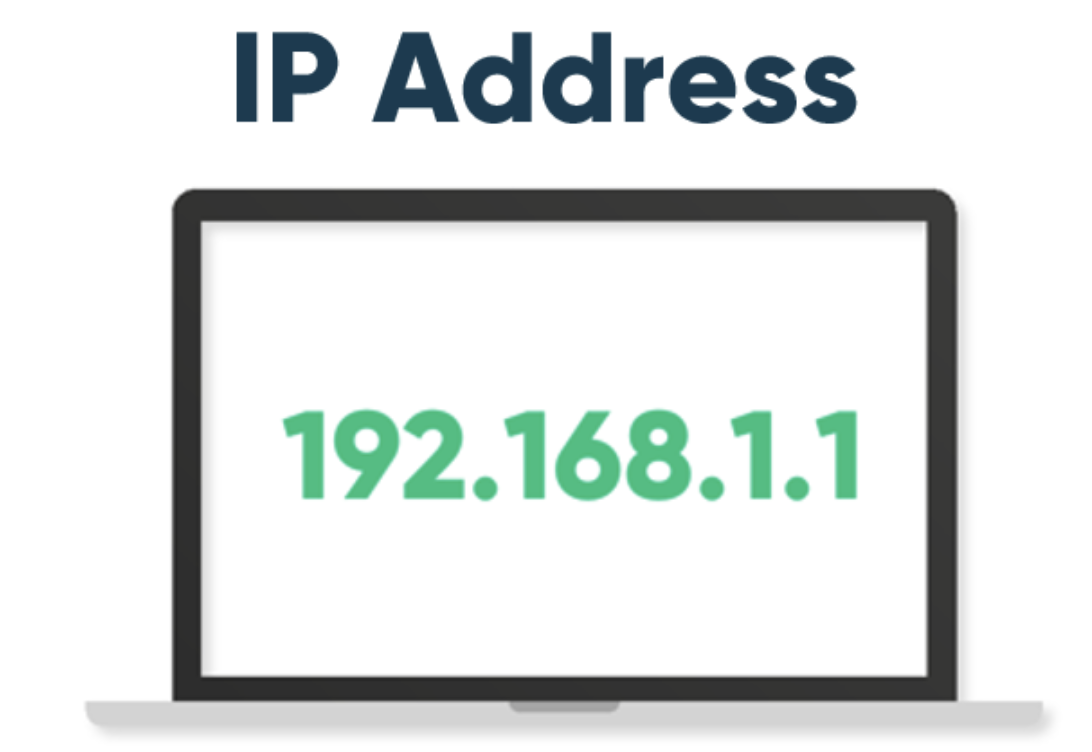
\includegraphics[width=\linewidth]{images/ip_address}
\end{columns}

\end{frame}




\begin{frame}{Zero factorial}

\colorbox{yellow!30}{\textbf{Poll.}} We define $0!=1$. Why?

\vfill 
\pause

\colorbox{green!30}{\textbf{Solution.}}  We give two arguments below 
\begin{enumerate}
\item \alert{By definition.} \pause  $0!$ gives the number of lists of length 0 whose elements are chosen from a pool of $0$ elements in which repetition is forbidden. \pause  There is only one such list: $()$, the empty list. 
\item \alert{Multiplicative identity.}  \only<5->{We would like $0!$ to equal the multiplicative identity (that is, 1).}  \only<6->{For example, consider the identity
\[ n! = n \times  (n-1)!\]
In the case where $n=1$, this becomes
\[1! = 1 \times 0!  \]
which holds only if $0!=1$.}
\end{enumerate}

\only<5>{\colorbox{red!30}{\textbf{Reference.}}  \begin{itemize}
\item \textit{1 is the multiplicative identity.}	 Multiplying some number $x$ by 1 leaves it unchanged.
\item \textit{0 is the additive identity.}	 Adding 0 to some number $x$ leaves it unchanged.
\end{itemize}
}
\end{frame}



\begin{frame}{Product notation}

We can write the factorial as 
\[ n! = \prod_{k=1}^n k,\]
which says to multiply all values of $k$ from $k=1$ to $k=n$.
\pause  
\vfill 
The right-hand side uses \alert{product notation}, which is useful more generally.
\pause 
\vfill 

\colorbox{yellow!30}{\textbf{Example.}} Try to compute $\prod_{k=1}^3 (2k+5)$ on your own.
\pause 
\vfill 
\colorbox{green!30}{\textbf{Solution.}} $\prod_{k=1}^3 (2k+5) = (7)(9)(11) =693.$

\pause 
\vfill 
\colorbox{red!30}{\textbf{Remark.}} Products of the form $\prod_{k=1}^0 k$ are called \underline{empty products}. These evaluate to 1. 

\end{frame}




\end{document}
